%
% geometrie.tex %% Beispiele partieller Differentialgleichungen
%
% (c) 2008 Prof Dr Andreas Mueller
%
\chapter{Geometrie der partiellen Differentialgleichungen erster Ordnung\label{chapter-geometrie}}
\lhead{Geometrie der L"osungen}
\begin{figure}
\begin{center}
\includegraphics[width=\hsize]{images/ode-1.pdf}
\end{center}
\caption{Richtungsfeld der gew"ohnlichen Differentialgleichung
$y'=-\frac16y+e^{-\frac{x}6}\cos x$ \label{geometrie:ode}}
\end{figure}
Bei gew"ohnlichen Differentialgleichungen kann man sich ein grobes
Bild des Verlaufs der L"osungen dadurch verschaffen, dass man
die von der Differentialgleichung vorgegeben Steigung der L"osungskurve
in jedem Punkt als Richtungsfeld aufzeichnet (Abbildung~\ref{geometrie:ode}).
Die gesuchte L"osung hat als Graphen eine Kurve, die in jedem Ihrer Punkte eine
Tangente hat, die mit dem gegebenen Richtungsfeld "ubereinstimmt.

Die L"osung einer
partiellen Differentialgleichung ist eine Funktion von mehreren Variablen,
bei zwei Variablen k"onnen wir den Graphen dieser Funktion als Fl"ache
"uber der $x$-$y$-Ebene visualisieren. Wie l"asst sich der Begriff der
Steigung "ubersetzen?


\section{Kurven auf der L"osungsfl"ache}
\rhead{Kurven auf der L"osungsfl"ache}
Die L"osungsfl"ache ist unausweichlich ein zweidimensionales
Objekt, dem nur mit partiellen Ableitungen beizukommen ist.
Die einzige M"oglichkeit, das Problem auf eine gew"ohnliche
Differntialgleichung zu reduzieren besteht darin, die L"osungsfl"ache
``kurvenweise'' zu finden, sie also also eine Schar von Kurven
zu betrachten.

\subsubsection{L"osungsfl"ache als Kurvenschar}
Der Graph der Funktion $u(x,y)$ kann auf zwei Arten als Schar von
Kurven betrachtet werden. Einerseits als durch die Werte $y$
parametrisierte Schar von Kurven $x\mapsto u(x,y)$, andererseits
also durch Werte $x$ parametrisierte Schar von Kurven $y\mapsto u(x,y)$.
Allerdings k"onnte auch jede andere Parametrisierung der Fl"ache
zu so einer Zerlegung Anlass geben. Die Parametrisierung
\begin{equation}
(s,t)\mapsto \vec x(s,t)
=
\begin{pmatrix}x(s,t)\\y(s,t)\\z(s,t)\end{pmatrix}
\label{quasilinear:kurvenschar}
\end{equation}
liefert die durch $s$ parametrisierte Schar $t\mapsto \vec x(s,t)$
von Kurven und die durch $t$ parametrisierte Schar $s\mapsto\vec x(s,t)$.

Umgekehrt beschreibt eine Schar von Kurven eine Fl"ache, die sich
in vielen F"allen wieder als Funktion $u(x,y)$ schreiben lassen wird.
Man muss dazu nur f"ur jeden Punkt $(x,y)$ die Gleichungen
\begin{align*}
x(s(x,y),t(x,y))&=x\\
y(s(x,y),t(x,y))&=y
\end{align*}
l"osen.
Die so bestimmten Funktionen $s(x,y)$ und $t(x,y)$ setzt man dann in
die Funktion $z(x,y)$ ein, und erh"alt die
L"osungsfunktion
\[
u(x,y)=z(s(x,y), t(x,y)).
\]
Das Ziel ist also, eine Schar (\ref{quasilinear:kurvenschar})
von Kurven zu finden, die alle auf der L"osungsfl"ache liegen.

\begin{beispiel}
Die Parametrisierung
\[
(\vartheta,\varphi)\mapsto
\begin{pmatrix}
\sin\vartheta\cos\varphi\\
\sin\vartheta\sin\varphi\\
\cos\vartheta
\end{pmatrix}
\]
beschreibt f"ur $0\le \vartheta\le \frac{\pi}2$
und $0\le\varphi\le 2\pi$ eine Halbkugel.

Die Kurvenscharen
\[
\vartheta\mapsto
\begin{pmatrix}
\sin\vartheta\cos\varphi\\
\sin\vartheta\sin\varphi\\
\cos\vartheta
\end{pmatrix}
\qquad
\text{und}
\qquad
\varphi\mapsto
\begin{pmatrix}
\sin\vartheta\cos\varphi\\
\sin\vartheta\sin\varphi\\
\cos\vartheta
\end{pmatrix}
\]
sind die durch $\varphi$, die geographische L"ange, parametrisierten
L"angen- und die durch $\vartheta$, die geographische Breite
parametrisierten Breitenkreise auf der Kugeloberfl"ache.

Die Gleichungen
\begin{align*}
x&=\sin\vartheta\cos\varphi\\
y&=\sin\vartheta\sin\varphi\\
\end{align*}
lassen sich mindestens f"ur $x\ne 0$ durch
\begin{align*}
\tan\varphi&=\frac{y}{x}\\
\sin\vartheta &=\sqrt{x^2+y^2}
\end{align*}
aufl"osen. Dies reicht bereits, um die Funktion $u(x,y)$
auszudr"ucken:
\[
u=\cos\vartheta=\sqrt{1-\sin^2\vartheta}=\sqrt{1-x^2-y^2}.
\]
\end{beispiel}

\subsubsection{Erster Parameter: Cauchy-Anfangswerte}
\begin{figure}
\begin{center}
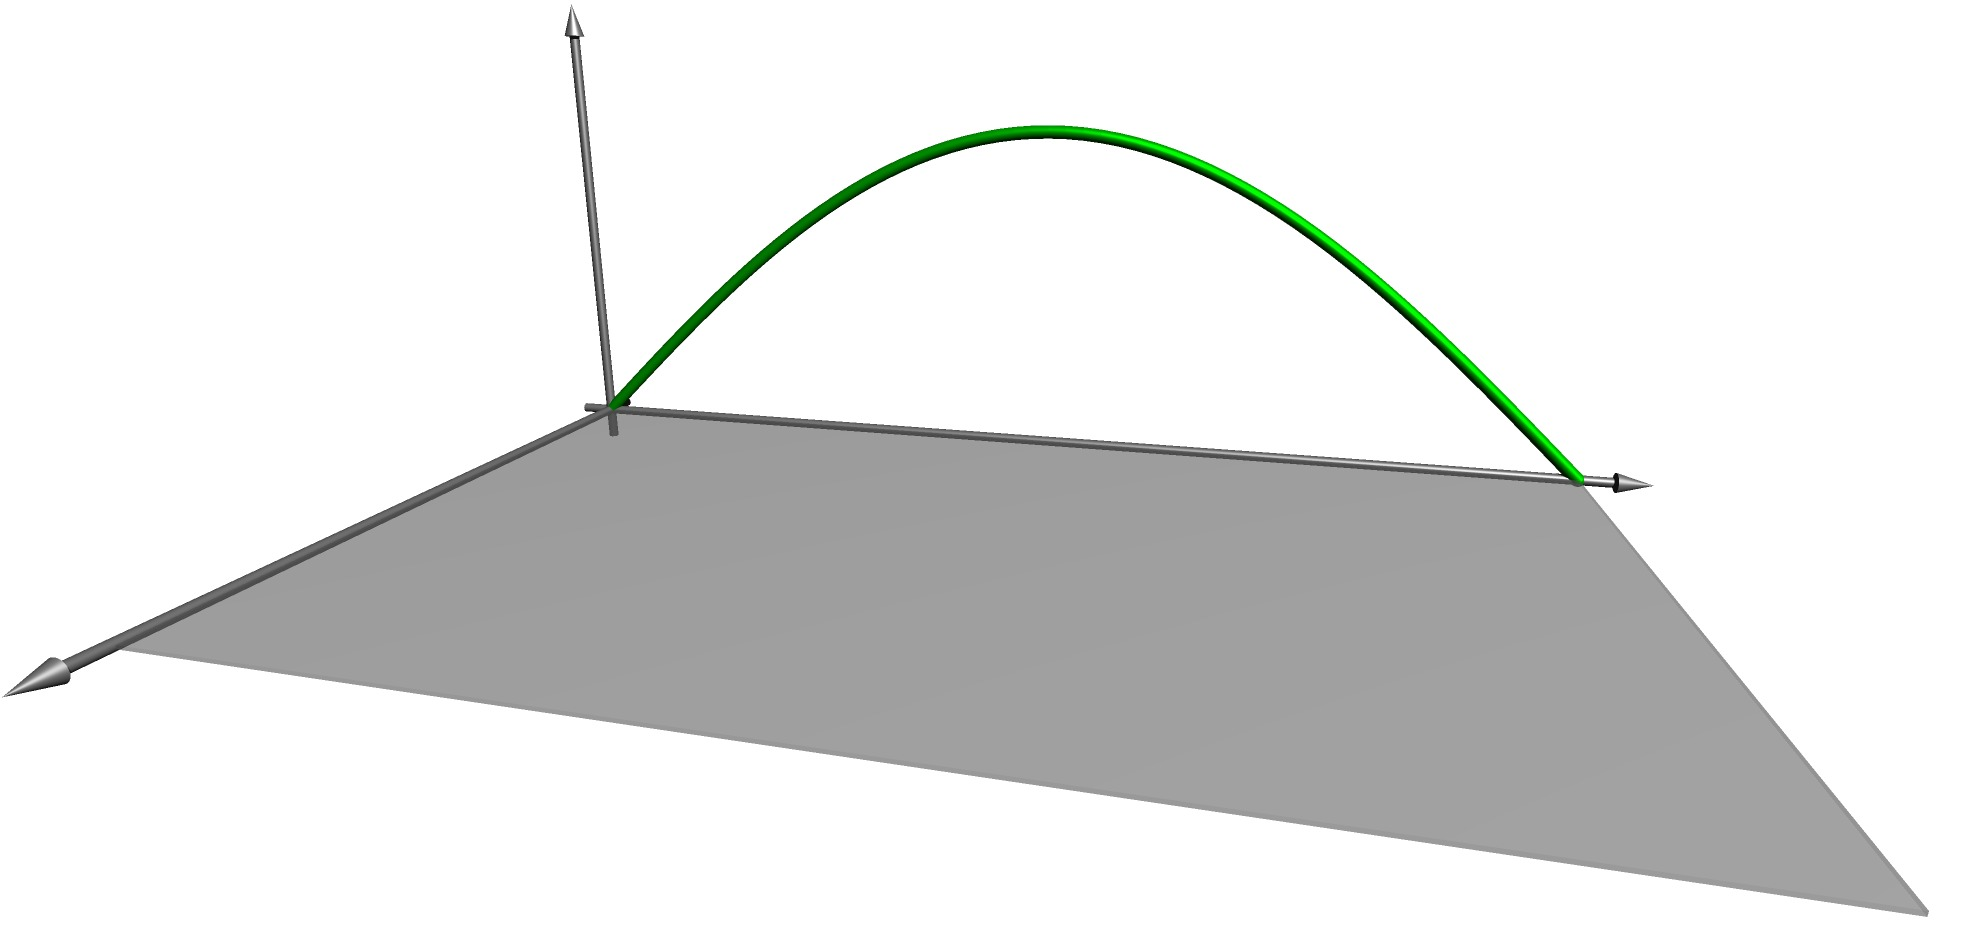
\includegraphics[width=\hsize]{3d/cauchy.jpg}
\end{center}
\caption{Cauchy-Anfangskurve f"ur eine partielle Differentialgleichung
($y$-Achse nach rechts)
\label{geometrie:cauchy-anfangskurve}}
\end{figure}
Wir wollen f"ur partielle Differentialgleichungen erster Ordnung
das Cauchy-Problem l"osen.
Das bedeutet, dass eine Anfangskurve bereits vorgegeben ist
(Abbildung~\ref{geometrie:cauchy-anfangskurve}).
Es gibt also eine Kurve
\begin{equation}
s\mapsto\vec x_0(s)=\begin{pmatrix}
x_0(s)\\
y_0(s)\\
z_0(s)
\end{pmatrix},
\label{quasilinear:anfangskurve}
\end{equation}
und die gesuchte L"osungsfunktion $u(x,y)$ muss f"ur jedes $s$ die
Bedingung
\[
u(x_0(s), y_0(s))=z_0(s)
\]
erf"ullen.
Man muss diese Kurve jetzt also erweitern zu einer Kurvenschar
der Form (\ref{quasilinear:kurvenschar}).
F"ur $t=0$ muss die Anfangskurve entstehen:
\[
\vec x(s,0)=x_0(s).
\]
Jede Scharkurve $t\mapsto \vec x(s,t)$ ist also eine Kurve
mit Anfangspunkt $x_0(s)$.
Es liegt nahe, solche Scharkurven als L"osungen von gew"ohnlichen
Differentialgleichungen zu finden.

\subsection{Quasilineare partielle Differentialgleichung erster Ordnung}
Wir betrachten in diesem Abschnitt eine quaslineare partielle 
Differentialgleichung
\begin{equation}
a\frac{\partial u}{\partial x}
+
b\frac{\partial u}{\partial y}
=
c.
\label{quasilinear:equation}
\end{equation}
Wir wollen zeigen, dass f"ur diese Art von Differentialgleichungen
das Cauchy-Problem meistens l"osbar ist, und wollen verstehen,
unter welchen Bedingungen es nicht l"osbar ist.

\subsubsection{Gew"ohliche Differentialgleichung erster Ordnung}
Wir erinnern uns zun"achst an die L"osung der gew"ohnlichen
Differentialgleichungen erster Ordnung.
Eine solche legt die Ableitung $y'$ in Abh"angigkeit von 
$(x,y)$ durch eine Funktion $f(x,y)$ fest: 
\[
y'=f(x,y).
\]
Gesucht ist dann eine Kurve $y(x)$, welche
in jedem Punkt $x$ die Steigung $y'(x)=f(x,y(x))$.
Geometrisch legt die Funktion $f(x,y)$ ein Richtungsfeld fest,
der Graph der L"osung ist eine Kurve, deren Tangente in jedem
Punkt mit dem Richtungsfeld zusammenf"allt.

Um eine L"osungskurve zu finden, kann man wie folgt vorgehen.
Die Anfgangswerte  $y(0)=y_0$ legen einen Punkt fest.
Die Differentialgleichung liefert jetzt die Steigung in
diesem Punkt: $y'(0)=f(0,y(0))$.
In erster N"aherung ist daher
\begin{equation}
y(h)=y(0)+f(0,y(0))\cdot h.
\label{quasilinear:euler}
\end{equation}
Mit $y(h)$ k"onnen wir das Verfahren wiederholen, und durch
wiederholte Anwendung von (\ref{quasilinear:euler})
nacheinander $y(2h)$, $y(3h)$,\dots bestimmen.
Nat"urlich ist dies nur ein N"aherungsverfahren, das "ubrigens
von Euler erdacht worden ist. Macht man $h$ sehr klein, wird
die Approximation der wahren L"osung immer besser.
Aber es macht plausibel, warum eine gew"ohnliche Differentialgleichung
erster Ordnung genau eine Anfangsbedingung braucht.

\subsubsection{L"osbarkeit}
Wir versuchen jetzt, diese "Uberlegung auf die L"osbarkeit einer
Differentialgleichung der Form (\ref{quasilinear:equation}) zu 
"ubertragen. Wir haben jetzt nat"urlich zwei partielle Ableitungen, die
durch die Gleichung (\ref{quasilinear:equation}) auch nicht
eindeutig bestimmt sind. Als lineare Gleichung f"ur die partiellen
Ableitungen betrachtet, hat (\ref{quasilinear:equation}) unendlich 
viele L"osungen.

Dies ist allerdings nicht so schlimm: denn wir m"ochten ja das Cauchy-Problem
l"osen: vorgegeben sind die Werte der Funktion entlang einer Kurve.
Wir haben also auch unendlich viele ``Anfangswerte''.
Zur Vereinfachung der Diskussion nehmen wir zun"achst an, dass die
Funktionswerte f"ur $x=0$ vorgeben sind.
Damit sind aber nicht nur die Funktionswerte $u(0,y)$ bekannt, sondern
auch die partiellen Ableitungen $\partial_yu(0,y)$.

Wenn der Koeffizient $a(x,y,u)$ von 
in (\ref{quasilinear:equation})
von $0$ verschieden ist, kann man die Gleichung
nach $\partial_xu$ aufl"osen.
Die eine partielle Ableitung legt also die andere fest.
Durch die Anfangswerte ist die eine partielle auf der
Anfangskurve bereits festgelegt, also steht auch schon fest,
die andere Ableitung ist daher auch bekannt. 

Wir sind also in einer "ahnlichen Situation wie bei gew"ohnlichen
Differentialgleichungen erster Ordnung: Wenn wir die 
Anfangskurve zum Beispiel f"ur $x=0$ kennen, also Werte
$u(0,y)$ bereits kennen, dann kennen wir
auch die Ableitungen, und k"onnen damit die L"osung
$y\mapsto u(h, y)$ f"ur ein kleines $h>0$ berechnen. Dies legt aber
wiederum die Ableitungen fest, so dass wir noch einen Schritt 
weiter zu $y\mapsto u(2h,y)$ gehen k"onnen sollten.
Indem wir so immer weiter schreiten, bekommen wir die ganze
L"osungsfunktion $u(x,y)$.

Wir erwarten daher, dass eine quasilineare partielle Differentialgleichung
nicht schwieriger zu l"osen ist, als eine gew"ohnliche Differentialgleichung
erster Ordnung.

\subsubsection{Vektorschreibweise der Differentialgleichung}
Die L"osung wird durch die folgende geometrische "Uberlegung vereinfacht.
Wir stellen dazu die gesuchte L"osungsfunktion $u(x,y)$ als Graph
in einem dreidimensionalen Koordinatensystem $x,y,u$ dar.
Die partielle Differentialgleichung (\ref{quasilinear:equation})
kann auch als Vektorgleichung
\begin{equation}
\begin{pmatrix}a\\b\\c\end{pmatrix}
\cdot
\begin{pmatrix}
\frac{\partial u}{\partial x}\\
\frac{\partial u}{\partial y}\\
-1
\end{pmatrix}
=0.
\label{quasilinear:vektorform}
\end{equation}
geschrieben werden, wie man sich durch Ausmultiplizieren "uberzeugen
kann.
Den linken Vektor bezeichnen wir mit
\[
\vec v=\begin{pmatrix}
a(x,y,u)\\
b(x,y,u)\\
c(x,y,u)
\end{pmatrix}.
\]
Der rechte Vektor
\[
\vec n=
\begin{pmatrix}
\frac{\partial u}{\partial x}\\
\frac{\partial u}{\partial y}\\
-1
\end{pmatrix}
\]
ist eine Normale auf den Graphen der Funktion
$z=u(x,y)$. Man kann sich von dieser Tatsache zum Beispiel so 
"uberzeugen: Die Tangentialvektoren in Achsrichtung sind
\[
\vec t_x
=
\begin{pmatrix}1\\0\\\frac{\partial u}{\partial x}\end{pmatrix}
\qquad
\text{und}
\qquad
\vec t_y
=
\begin{pmatrix}0\\1\\\frac{\partial u}{\partial y}\end{pmatrix}
\]
Das Skalarprodukt von $\vec n$ mit den Vektoren $\vec t_x$ und $\vec t_y$
ist:
\[
\vec n\cdot\vec t_x
=
\begin{pmatrix}
\frac{\partial u}{\partial x}\\
\frac{\partial u}{\partial y}\\
-1
\end{pmatrix}
\cdot
\begin{pmatrix}1\\0\\\frac{\partial u}{\partial x}\end{pmatrix}
=0
\qquad
\text{und}
\qquad
\vec n\cdot\vec t_y
=
\begin{pmatrix}
\frac{\partial u}{\partial x}\\
\frac{\partial u}{\partial y}\\
-1
\end{pmatrix}
\cdot
\begin{pmatrix}0\\1\\\frac{\partial u}{\partial y}\end{pmatrix}
=0.
\]
\begin{figure}
\begin{center}
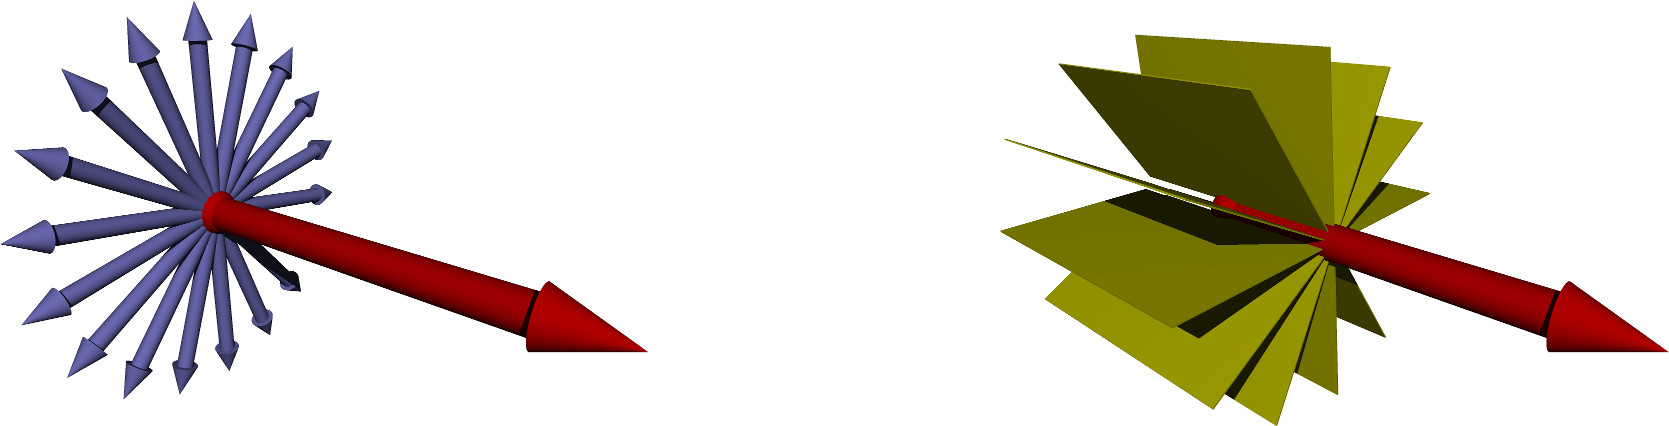
\includegraphics[width=\hsize]{3d/normals.jpg}
\end{center}
\caption{Die Normalen der L"osungsfl"ache einer quasilinearen
partiellen Differentialgleichung erster Ordnung sind alle senkrecht
auf dem Vektor $\vec v$ (rot, linkes Bild). Die Tangentialebenen an
die L"osungsfl"ache haben daher eine gemeinsame Gerade mit Richtung $\vec v$.
\label{geometrie:normals}}
\end{figure}%
Die Gleichung (\ref{quasilinear:vektorform}) sagt also,
dass diese Normale senkrecht auf dem Vektor $\vec v$ steht.
Gesucht ist also eine Fl"ache, deren Normale senkrecht auf dem
Vektor $\vec v$ steht. Die m"oglichen Tangentialebenen von L"osungen
haben also die Gerade mit Richtung $\vec v$ gemeinsam
(Abbildung~\ref{geometrie:normals}).
Sie bilden ein B"uschel von Ebenen.

Wir verstehen jetzt, wie wir das Bild, das wir uns von den gew"ohnlichen
Differentialgleichungen gemacht haben, f"ur partielle Differentialgleichungen
modifizieren m"ussen. Die Differentialgleichung gibt in jedem Punkt
des Raumes ein B"uschel von Ebenen vor, welche als Tangentialebenen der
L"osungsfl"ache in Frage kommen. Die Richtung der Anfangskurve w"ahlt aus
diesem B"uschel ein Tangentialebene aus, die Tangentialebene in einem 
Punkt der Anfangskurve muss die Tangente der Anfangskurve enthalten
\begin{figure}
\begin{center}
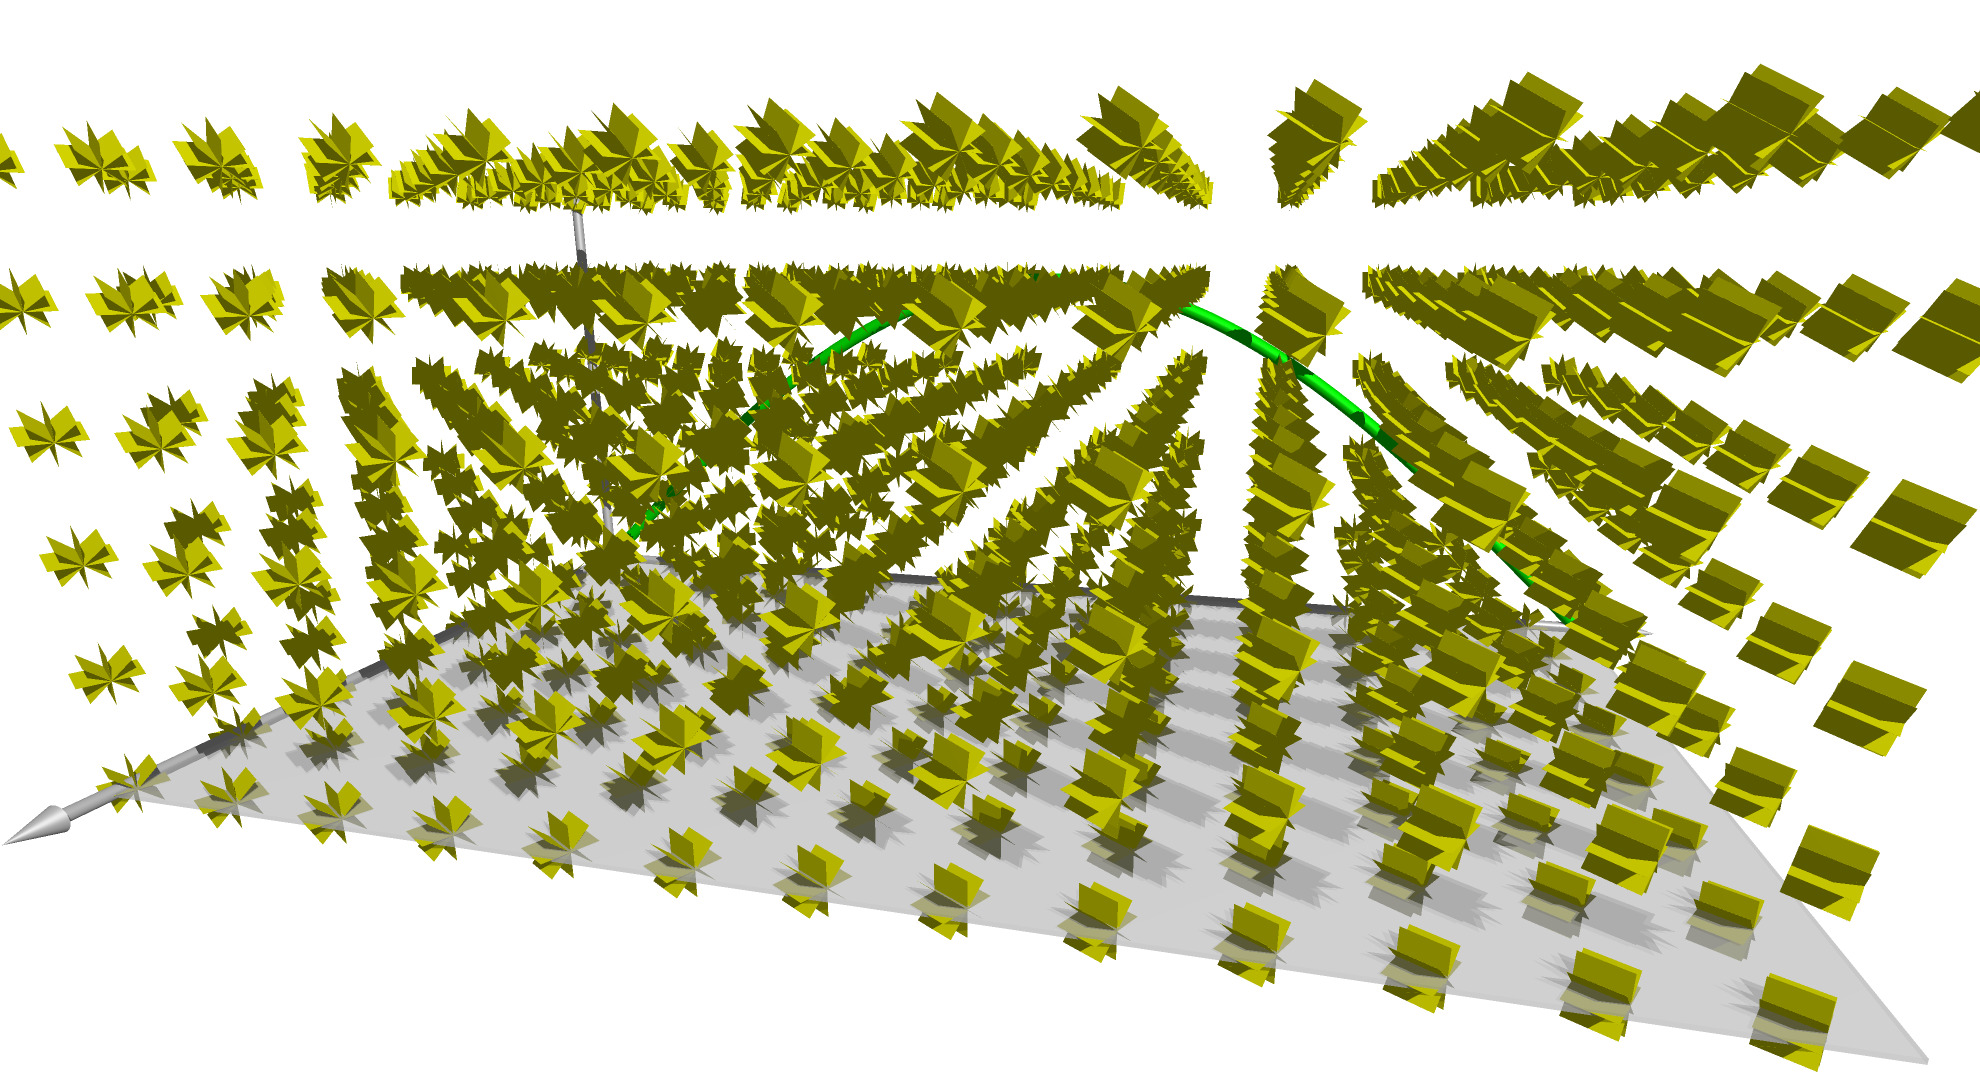
\includegraphics[width=\hsize]{3d/planes.jpg}
\end{center}
\caption{Feld von Ebenenb"uscheln, definiert durch eine quasilineare
partielle Differentialgleichung erster Ordnung
\label{geometrie:ebenenbueschelfeld}}
\end{figure}
(Abbildung~\ref{geometrie:ebenenbueschelfeld}).

Das bedeutet zum Beispiel auch, dass die Schnittkurve von
zwei L"osungsfl"achen immer $\vec n$ als Tangente haben muss.
Kurven, die in jedem Punkt die Richtung $\vec n$ haben, sind
als von ganz besonderer Bedeutung.
Die Vektoren
\[
(x,y,u)\mapsto
\vec v=
\begin{pmatrix}
a(x,y,u)\\b(x,y,u)\\c(x,y,u)
\end{pmatrix}
\]
bilden ein Vektorfeld, welches in jedem Punkt tangential
an die gesuchte Fl"ache verl"auft.

\subsubsection{Charakteristiken}
Statt direkt die L"osungsfl"ache zu suchen, k"onnen wir das Vektorfeld
$\vec v$ dazu verwenden, einzelne Kurven in der L"osungsfl"ache
zu bestimmen.
\begin{figure}
\begin{center}
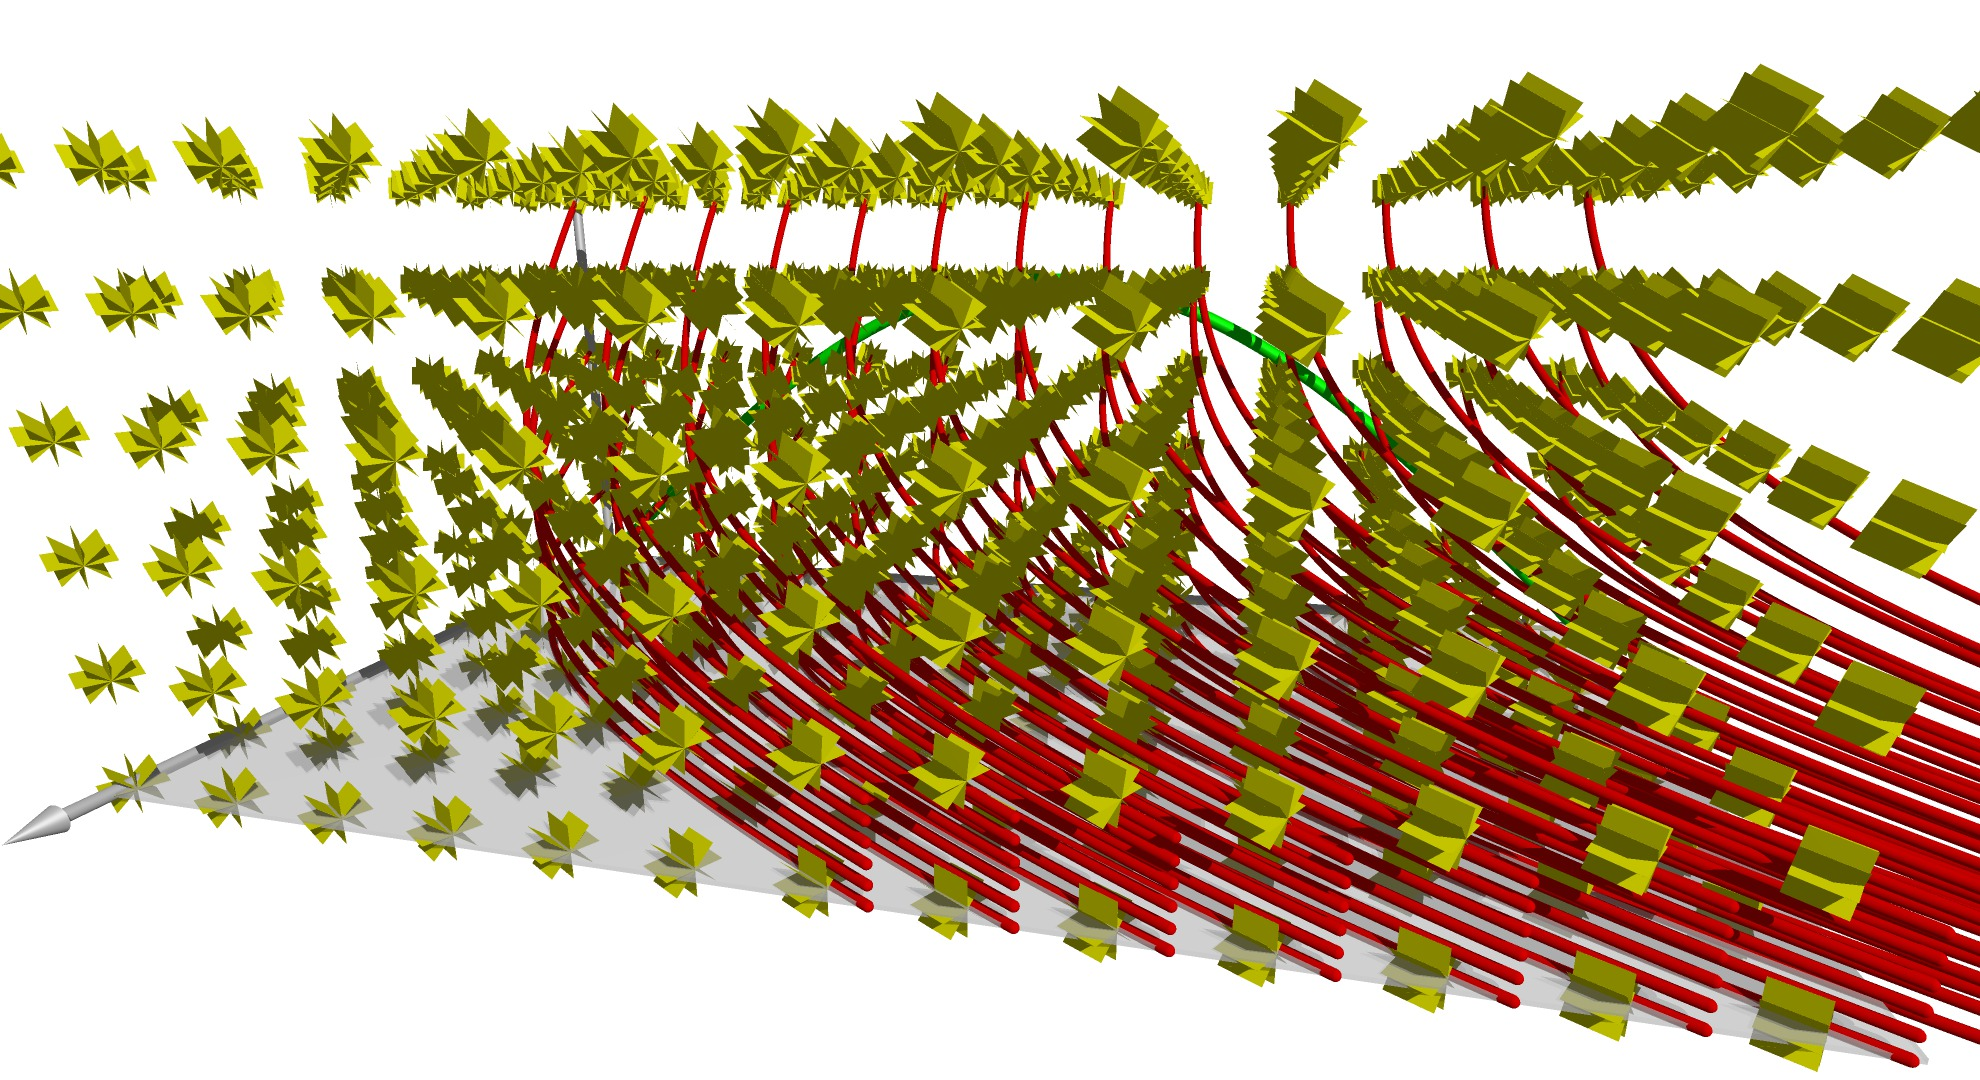
\includegraphics[width=\hsize]{3d/chrpl.jpg}
\end{center}
\begin{center}
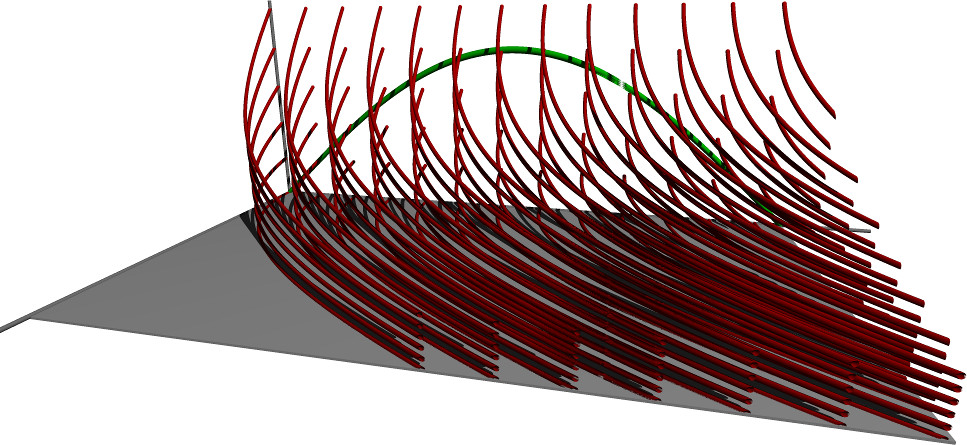
\includegraphics[width=\hsize]{3d/chr.jpg}
\end{center}
\caption{Charakteristiken einer quasilinearen partiellen Differentialgleichung
erster Ordnung, mit eingezeichneten Ebenenb"uscheln (oben) und nur die
Charakteristiken (unten)\label{geometrie:charekeristiken-mit-buescheln}}
\end{figure}
Ist ein Punkt der Fl"ache bekannt,
kann man davon ausgehend eine L"osungskurve des Vektorfeldes konstruieren.
Dazu muss man die gew"ohnliche Differentialgleichung
\begin{equation}
\frac{d}{dt}\begin{pmatrix}x(t)\\y(t)\\z(t)\end{pmatrix}
=
\begin{pmatrix}
a(x(t),y(t),u(t))\\b(x(t),y(t),u(t))\\c(x(t),y(t),u(t))
\end{pmatrix}
\label{quasilinear:charakteristik}
\end{equation}
l"osen.
Eine L"osungskurve von (\ref{quasilinear:charakteristik}) ist in jedem
Punkt tangential an die L"osungsfl"ache, sie verl"asst die Fl"ache also
nicht.

\begin{definition}
\label{def:quasiliniear:charakteristik}
\index{Charakteristik!einer quasilinearen partiellen
Differentialgleichung erster Ordnung}
Die L"osungskurven der gew"ohnlichen Differentialgleichung
(\ref{quasilinear:charakteristik}) heissen Charakteristiken
der partiellen Differentialgleichung (\ref{quasilinear:equation}).
\end{definition}

\subsubsection{L"osung des Cauchy-Problems}
\begin{figure}
\begin{center}
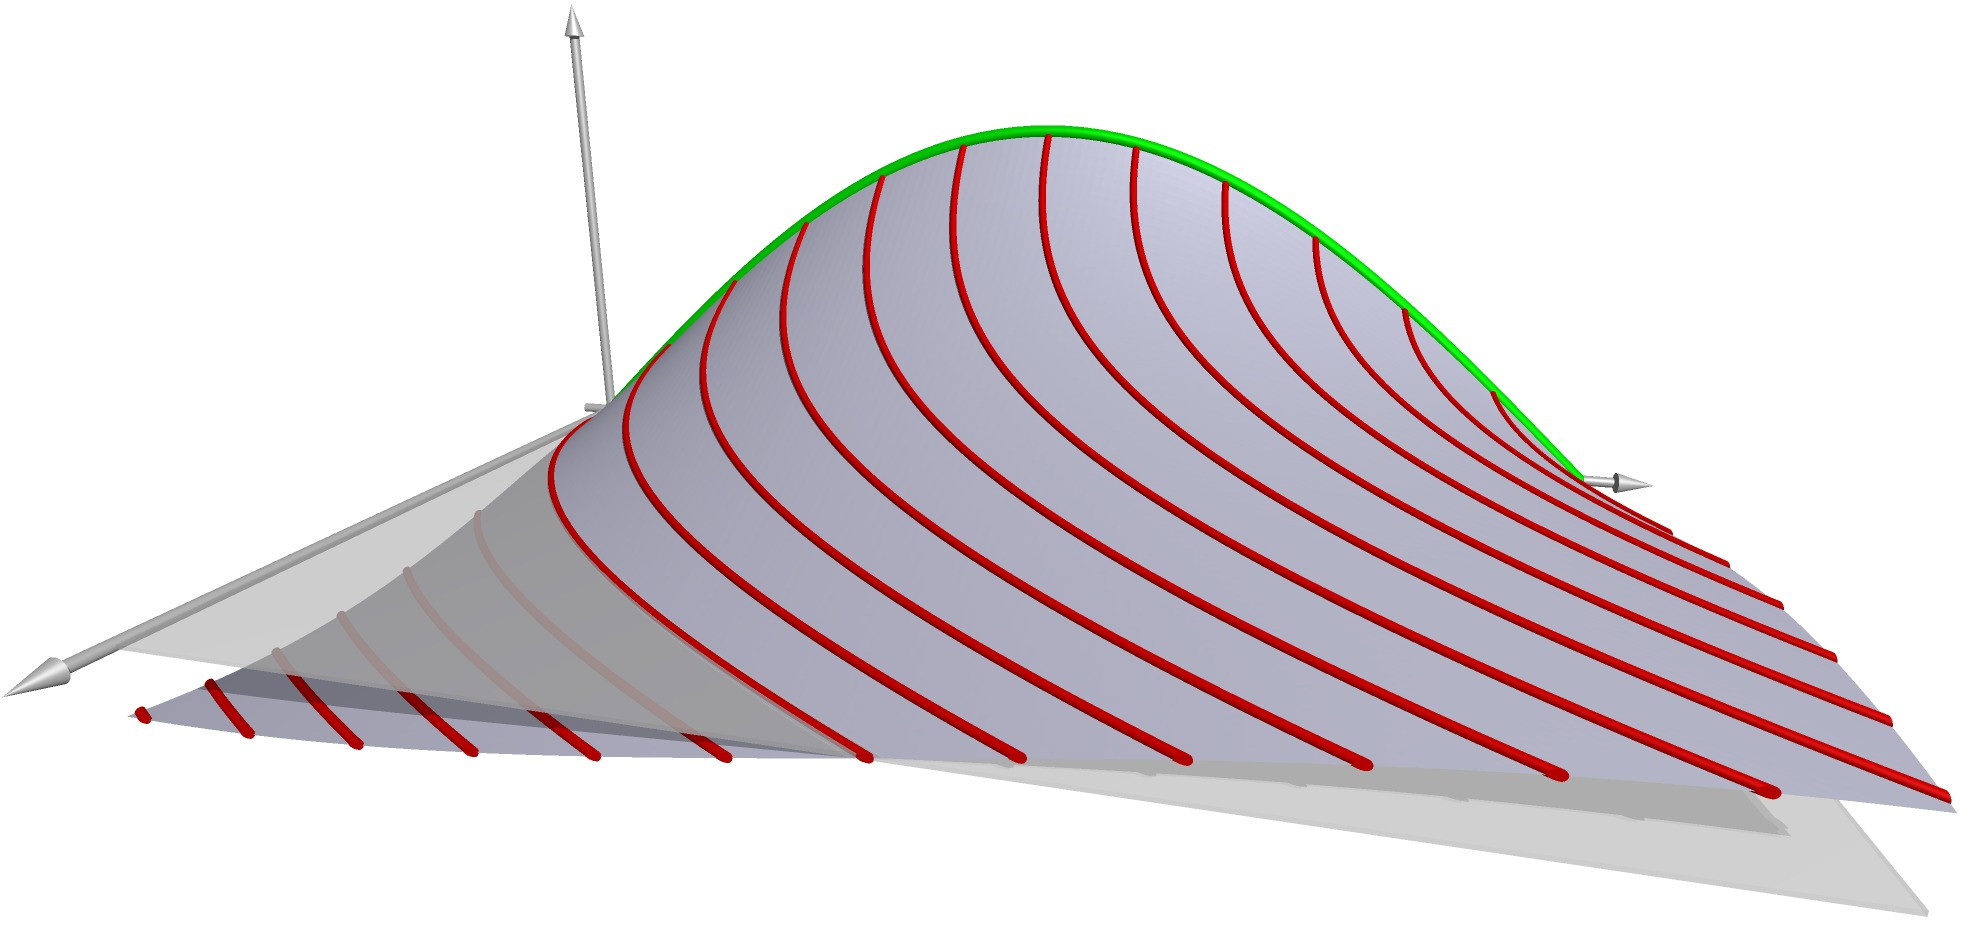
\includegraphics[width=\hsize]{3d/sol.jpg}
\end{center}
\caption{L"osung einer quasilinearen partiellen Differentialgleichung
erster Ordnung: die L"osungsfl"ache wird von Charakteristiken (rot) gebildet,
sie ist parametrisiert durch den Parameter der Anfangskurve (gr"un) und den
Kurvenparamter entlang der Charakteristik.
\label{geometrie:loesung-mit-charakteristiken}}
\end{figure}
Das Cauchy-Problem l"asst sich jetzt mit Hilfe von Charakteristiken
l"osen. Die L"osungsfl"ache besteht aus Charakteristiken, die auch
die Anfangskurve schneiden
(Abbildung~\ref{geometrie:loesung-mit-charakteristiken}).
Um die L"osung zu berechnen, ist also wie folgt vorzugehen:
\begin{enumerate}
\item
F"ur jedes $s$ ist die Differentialgleichung der Charakteristiken
(\ref{quasilinear:charakteristik}) zu l"osen und eine 
L"osungskurve $t\mapsto \vec x(s,t)$ zu finden, die
die Anfangsbedingung $\vec x(s,0)=\vec x_0(s)$ erf"ullt.
\item 
Aus den Gleichungen (\ref{quasilinear:kurvenschar}) f"ur die
Kurvenschar m"ussen die Parameter $s$ und $t$ eliminiert werden,
sie muss in die Form $z=u(x,y)$ umgeformt werden.
\end{enumerate}

Sind die Koeffizienten der Differentialgleichung differenzierbare Funktionen,
dann ist das Vektorfeld differenzierbar.
Ist auch die Anfangsbedingung differenzierbar,
dann besagen die allgemeinen S"atze "uber die Abh"angigkeit der L"osung einer
gew"ohnlichen Differentialgleichung von den Anfangsbedingungen, dass die so
konstruierte L"osungsfl"ache differenzierbar ist.

Insgesamt haben wir damit das Problem der L"osung der partielle Differentialgleichungen auf das Problem 
zur"uckgef"uhrt, beliebige L"osungskurven eines Vektorfeldes, also auf
eine gew"ohnliche Differentialgleichung zur"uckgef"uhrt.


\subsubsection{Welche Anfangskurven sind nicht geeignet?}
Damit das eben skizzierte L"osungsverfahren funktioniert, 
darf die Anfangskurve keine Charakteristik sein.
Andernfalls erh"alt man ja durch Berechnung der von einem Punkt
der Anfangskurve ausgehenden Charakteristik nur wieder die
Anfangskurve, es entsteht gar keine Fl"ache.

Damit liefern uns die Charakteristiken nicht nur ein Verfahren
zur L"osung einer partiellen Differentialgleichung erster Ordnung,
sondern auch ein Verfahren um zu entscheiden, wo Anfangswerte
vorgegeben werden m"ussen.

Sei die partielle Differentialgleichung auf dem Gebiet $\Omega$
definiert.
Eine Charakteristik ausgehend von einem Randpunkt mit vorgegebenem
Randwert wird sich zun"achst durch das Gebiet bewegen, kann dieses
aber in einem anderen Punkt auch wieder verlassen. Der Wert der
L"osungsfunktion in diesem zweiten Randwert ist offenbar durch die
Vorgabe des ersten Randwertes bereits festgelegt.
Eine andere Vorgabe w"urde verhindern, dass das Problem "uberhaupt
eine L"osung hat.

Randwerte m"ussen also auf einer Teilmenge $M\subset\partial \Omega$
festgelegt werden so, dass jede Charakteristik nur einen Punkt der
Menge $M$ trifft.

\subsection{Beispiele}
In diesem Abschnitt rechnen wir ein paar Beispiel f"ur das eben
skizzierte L"osungsverfahren durch.
\subsubsection{Konstante Koeffizienten\label{konstantekoeff}}
Wir betrachten die Differentialgleichung
\[
\frac{\partial u}{\partial x}+2\frac{\partial u}{\partial y}=3
\]
mit der Anfangsbedingung $u(0,y)=\sin y$ und m"ochten eine L"osung f"ur
$x>0$ finden.

Die Anfangskurve mit Parameter $s$ hat die Form
\[
\vec x_0(s)
=
\begin{pmatrix}
0\\s\\\sin s
\end{pmatrix}.
\]
Wir m"ussen also eine Kurvenschar finden, die von dieser Anfangskurve
ausgeht.

Die Differentialgleichung der Charakteristiken ist
\[
\frac{d}{dt}\begin{pmatrix}x(t)\\y(t)\\z(t)\end{pmatrix}
=
\begin{pmatrix}1\\2\\3\end{pmatrix},
\]
sie hat die L"osungskurven
\[
t\mapsto\begin{pmatrix}x_0\\y_0\\z_0\end{pmatrix}+t\begin{pmatrix}1\\2\\3\end{pmatrix}
\]
Der Anfangspunkt $(0,s,\sin s)$ entwickelt sich also mit der Zeit zu
\[
\begin{pmatrix}
x(s,t)\\
y(s,t)\\
z(s,t)
\end{pmatrix}
=
\begin{pmatrix}0\\s\\\sin s\end{pmatrix}+t\begin{pmatrix}1\\2\\3\end{pmatrix}
=
\begin{pmatrix}
t\\
s+2t\\
\sin s+3t
\end{pmatrix}.
\]
Diese Kurvenschar beschreibt die L"osungsfl"ache, wir m"ochten daraus aber
wieder die L"osung in der vertrauteren Form $u(x,y)$ gewinnen.
Dazu m"ussen die Variablen $s$ und $t$ aus den Gleichungen
\begin{align*}
x&=t\\
y&=s+2t\\
z&=\sin s+3t
\end{align*}
eliminiert werden.
Aus der ersten Gleichung folgt, dass $t$ einfach durch $x$ ersetzt werden
kann.
Aus der zweigen Gleichung folgt dann, dass $s=y-2x$.
Setzt man dies in der dritten Gleichung ein, erh"alt man $z=\sin(y-2x)+3t$.
Die L"osung der Differentialgleichung ist also
\[
u(x,y)=\sin(y-2x)+3x.
\]
Durch Einsetzen in die Differentialgleichung und die Randbedingung
kann man sich davon "uberzeugen, dass dies tats"achlich eine L"osung
ist:
\begin{align*}
\frac{\partial u}{\partial x}
&=-2\cos(y-2x)+3
\\
\frac{\partial u}{\partial y}
&=\cos (y-2x)
\\
\Rightarrow\qquad
\frac{\partial u}{\partial x}
+2
\frac{\partial u}{\partial y}
&=
-2\cos(y-2x)+3
+2\cos(y-2x)=3
\\
u(0,y_0)&=\sin y_0.
\end{align*}

\subsubsection{Kreisf"ormige Charakteristiken}
Wir l"osen die Differentialgleichung
\[
y\frac{\partial u}{\partial x}-x\frac{\partial u}{\partial y}=0
\]
Gem"ass der Methode der Charakteristiken m"ussen wir die L"osungskurven
des Vektorfeldes
\[
\begin{pmatrix}
y\\-x\\0
\end{pmatrix}
\]
finden. Da die $z$-Komponente verschwindet, sind die $z$-Komponenten
der L"osungskurven konstant, wir ignorieren sie daher in der nachstehenden
Rechnung.

L"osungen f"ur das Vektorfeld 
\[
\begin{pmatrix}
y\\-x
\end{pmatrix}
\]
in der Ebene sind Funktionen $x(t)$ und $y(t)$, welche die Gleichungen
\begin{align*}
\dot x(t)&=y(t)\\
\dot y(t)&=-x(t)
\end{align*}
erf"ullen. Leitet man die erste Gleichung ab, und setzt die zweite
darin ein, erh"alt man die Differentialgleichung zweiter Ordnung
\[
\ddot x(t)=-x(t)
\]
mit den bekannten L"osungen $a\cos t$ und $a \sin t$. Da die L"osungskurve
zur Zeit $t=0$ auf der $y$-Achse beginnen soll, muss sie in Vektorschreibweise
\[
\begin{pmatrix}
x(t)\\y(t)
\end{pmatrix}
=y_0\begin{pmatrix}
\sin t\\
\cos t
\end{pmatrix}
\]
sein, die Kurven sind also Kreise mit Radius $y_0$ um den Nullpunkt. Offenbar
k"onnen wir jeden Punkt der Ebene von einem Punkt in der Halbgeraden
$\{(0,y_0)|y_0 <0\}$ aus erreichen, die Anfangsbedingung muss also nur f"ur
$y_0<0$ spezifiziert werden.

Die L"osung zur Anfangsbedingung $g(y)$ kann jetzt wie folgt bestimmt werden.
Zu einem Punkt $(x,y)$ m"ussen $y_0$ und $t$ gefunden werden, davon brauchen wir
jedoch nur den Betrag, also $y_0=-\sqrt{x^2+y^2}$. Die L"osung ist also
\[
u(x,y)=g(-\sqrt{x^2+y^2}).
\]

Aus diesem Beispiel k"onnen wir mehrere Lehren ziehen: 
\begin{enumerate}
\item Dass Festlegung einer Anfangsbedingung f"ur $y_0>0$ nicht n"otig ist,
kann man der Differentialgleichung in unmittelbarer N"ahe der $y$-Achse nicht
ansehen, erst der Verlauf der Charakterisitiken im Grossen erm"oglicht
diese Erkenntnis. Dieses Ph"anomen wird durch den ``zus"atzlichen Platz''
erm"oglicht, den der zweidimensionale Definitionsbereich der partielle Differentialgleichung gegen"uber dem
eindimensionalen Definitionsbereich der gew"ohnlichen DGL bietet.
\item Der Punkt $(0,0)$ hat spezielle Eigenschaften: wenn die L"osung stetig
sein soll, muss $g(0)=\lim_{y\to 0-} g(y)$ sein. Damit die L"osung differenzierbar
wird, muss aber zus"atzlich $g'(x)=0$ sein.
\end{enumerate}

\subsubsection{Ein nicht l"osbares Anfangswertproblem\label{unloesbar}}
Die Differentialgleichung
\[
x\frac{\partial u}{\partial x}
+
y\frac{\partial u}{\partial y}
=0
\]
soll zu den Anfangsbedingungen $u(0,y)=\sin y$ gel"ost werden.
Dazu berechnen wir wieder zuerst die Charakteristiken (ohne die 
$z$-Komponente, die wieder konstant ist)
\[
\frac{d}{dt}
\begin{pmatrix}
x(t)\\y(t)
\end{pmatrix}
=
\begin{pmatrix}
x(t)\\y(t)
\end{pmatrix}
\quad
\Rightarrow
\quad
\left\{
\begin{aligned}
\dot x(t)&=x(t)\\
\dot y(t)&=y(t)
\end{aligned}
\right.
\]
Die L"osungskurven sind Strahlen durch den Ursprung:
\[
\begin{pmatrix}
x(t)\\y(t)
\end{pmatrix}
=\begin{pmatrix}x_0\\y_0\end{pmatrix}e^t
\]
Um die L"osung zu konstruieren, m"ussen wir jetzt zu einem Punkt
$(x,y)$ den Anfangspunkt der zugeh"origen Charakteristik auf der $y$-Achse
finden. Da alle Charakteristiken durch den Nullpunkt gehen, ist dies 
gar nicht m"oglich. 

Das Problem r"uhrt daher, dass wir die Anfangsbedinung selbst auf einer
Charakteristik festgelegt haben, die Charakteristiken sind also als
Anfangskurven ungeeignet. Nur wenn die Anfangsbedingung auf einer Kurve
festgelegt wird, die transversal, also nirgends tangential, zu den
Charakteristiken verl"auft, kann das Anfangswertproblem gel"ost werden.

\subsection{Allgemeine partielle Differentialgleichungen erster Ordnung}
Als Beispiel betrachten wir die folgende partielle Differentialgleichung
erster Ordnung f"ur die Funktion $u(x,y)$
\begin{equation}
F\biggl(
x,y,u(x,y),\frac{\partial u}{\partial x},\frac{\partial u}{\partial y}
\biggr)=0.
\end{equation}
Diese Gleichung beschreibt einen impliziten Zusammenhang zwischen
dem Ort im $x$-$y$-$u$-Koordinatensystem und den beiden Steigungen
$\partial_xu$ und $\partial_yu$.

Ein Anfangswertproblem, bei dem die Anfangswerte f"ur $x=0$ als
Funktion $g(y)$ festgelegt sind, also
\[
u(0,y)=g(y),
\]
legt auch die
partiellen Ableitungen $\partial_y u(0,y)=g'(y)$ fest.  Die partielle
Differentialgleichung schr"ankt damit ein, welche m"oglichen Ableitungen
$\partial_xu(0,y)$ m"oglich sein. Oft wird dies nicht eindeutig sein,
die Steigung in $x$-Richtung kann also verschiedene Werte annehmen,
es kann verschiedene L"osungsfunktionen geben. "Ahnlich wie bei der
L"osung gew"ohnlicher Differentialgleichungen ist zu jedem Wert
aus der bereits bekannten partiellen Ableitung $\partial_yu(x,y)$
die Steigung $\partial_xu(x,y)$ bestimmt, es ist somit plausibel, dass
sich die L"osung "ahnlich wie bei der L"osung gew"ohnlicher Differentialgleichungen
entwickeln l"asst. In voller Allgemeinheit ist dies nicht ganz einfach,
und f"ur unsere Zwecke auch nicht notwendig, denn alle wesentlichen
Eigenschaften lassen sich an dem einfacheren Fall der quasilinearen
partielle Differentialgleichung auch beobachten.


\section{Entstehung von Singularit"aten}
Die L"osung einer partiellen Differentialgleichung h"angt entscheidend
vom Verlauf der Charakteristiken ab. Treffen sich zwei Charakteristiken
in einem Punkt, ist die L"osung nicht eindeutig bestimmt. Die L"osung
ist also nur solange bestimmt, als sich die Charakteristiken nicht "uberschneiden.
Andernfalls treten Singularit"aten in der L"osung auf.

Als Beispiel betrachten wir die nichtlineare Gleichung 
\begin{equation}
\frac{\partial u}{\partial t}+u\frac{\partial u}{\partial x}=0.
\label{wellenichtlinear}
\end{equation}
mit der Anfangsbedingung 
\[
u(0,x_0)=g(x_0)=e^{-4(x_0-\frac12)^2}.
\]
Nach der Methode der Charakterisitiken brauchen wir eine L"osungskurve
des Vektorfeldes
\[
\begin{pmatrix}
1\\
u\\
0
\end{pmatrix}
\]
durch den Punkt $(0,x_0, z_0)$, also eine L"osung des Differentialgleichungssystems
\[
\left.
\begin{aligned}
\frac{d}{d\tau} t(\tau)&=1\\
\frac{d}{d\tau} x(\tau)&=z(\tau)\\
\frac{d}{d\tau} z(\tau)&=0
\end{aligned}
\quad
\right\}
\qquad
\Rightarrow
\qquad
\left\{
\quad
\begin{aligned}
t(\tau)&=\tau\\
z(\tau)&=z(0)\\
x(\tau)&=z(0)\tau +x(0)
\end{aligned}
\right.
\]
Der Parameter $\tau$ hat also die Bedeutung von $t$.
Die L"osungsfl"ache ist somit
\[
(t,x_0)\mapsto
\begin{pmatrix}
t\\
g(x_0)t+x_0\\
g(x_0)
\end{pmatrix}.
\]
Die Charakteristiken in der $x$-$y$-Ebene sind Geraden mit einer
Steigung, die von $g(x_0)$ abh"angt. Je gr"osser $g(x_0)$ ist, desto
``schneller'' bewegt sich die Integralkurve nach ``rechts''. Grosse
Werte der Anfangsbedingung k"onnen also die kleinen Wert "uberholen,
dabei entsteht eine Singularit"at.

Zur Zeit $t$ hat die L"osungsfunktion die Parameterdarstellung
\[
x_0\mapsto (g(x_0)t+x_0,g(x_0))
\]
die Graphen in Abbildung~\ref{g} zeigen, wie sich die L"osungskurve
mit zunehmender Zeit entwickelt.
Es ist offensichtlich, dass f"ur gen"ugend grosse Zeit $t$ die
L"osungsfl"ache nicht mehr als Graph einer Funktion $u(t,x)$ derstellbar ist.
\begin{figure}
\begin{center}
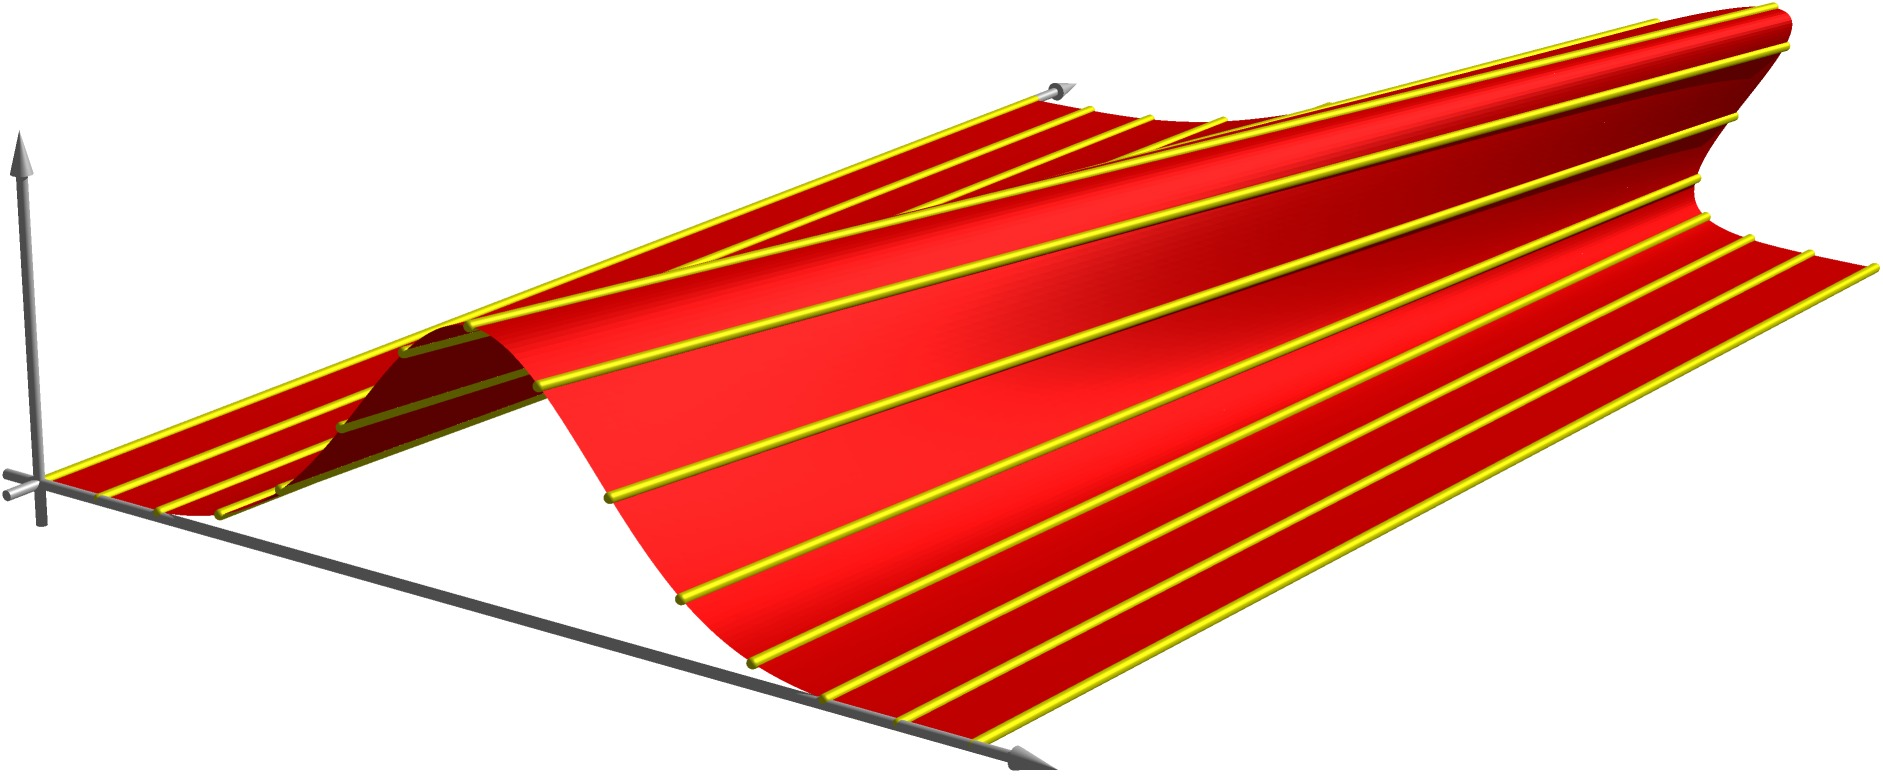
\includegraphics[width=\hsize]{graphics/welle}
\end{center}
\caption{L"osung der Differentialgleichung (\ref{wellenichtlinear}) mit
entstehender Singularit"at\label{g}}
\end{figure}

\section{Randbedingungen}
Die Methode der Charakterisitiken erlaubt uns herauszufinden, auf welchen
Teilen des Randes die Werte einer L"osunge einer partiellen
Differentialgleichung vorgegeben werden m"ussen.
Die L"osungsfl"ache $u(x,y)$ besteht ja aus Charatkeristiken, sie ist also
genau dann vollst"andig bestimmt, wenn jede Charakteristik durch mindestens 
einen vorgegebenen Randpunkt verl"auft.

F"ur die Differentialgleichung
\[
\frac{\partial u}{\partial x}+2\frac{\partial u}{\partial y}=3
\]
hatten wir die Charakterisiken 
\[
t\mapsto\begin{pmatrix}x_0\\y_0\\z_0\end{pmatrix}+t\begin{pmatrix}1\\2\\3\end{pmatrix}
\]
gefunden. Eine L"osungsfunktion $u(x,y)$ muss von Charakteristiken
"uberdeckt werden. 
Die Projektionen dieser Kurven in die $x$-$y$-Ebene sind Geraden
mit Steigung $2$. Der Rand des Gebietes $\Omega$, in dem die Gleichung gel"ost
werden soll, muss also jede Gerade mit Steigung $2$ h"ochstens einmal
schneiden.

Das Gebiet $\{(x,y)\in\mathbb R^2\,|\, x >0\}$  aus \ref{konstantekoeff}
hat die $x$-Achse als Rand, und diese schneidet jeder Gerade mit Steigung
$2$ genau einmal.

Interessanter wird die Diskussion jedoch f"ur das Gebiet
$\Omega=\{(x,y)\,|\,0<x,y<1\}$. Die Abbildungen \ref{geometrie:charrand1}
bis \ref{geometrie:charrand3} zeigen verschiedene M"oglichkeiten:
\begin{enumerate}
\item
In Abbildung~\ref{geometrie:charrand1} sind Randwerte auf dem linken
und rechten Rand vorgegeben. Offenbar reichen diese Randwerte nicht, um
die Funktionswerte "uberall im Gebiet eindeutig zu bestimmen, es bleibt
ein Teilgebiet, in dem die L"osungsfunktion nicht festgelegt ist.
\item
In Abbildung~\ref{geometrie:charrand2}
sind die Randwerte am oberen und unteren Rand vorgegeben.
In diesem Fall sind die Randwerte "uberbestimmt, eine L"osung ist
nur m"oglich, wenn die Werte auf der linken H"alfte des unteren
Randes mit den Werten auf der rechten H"alfte des oberen Randes
kompatibel sind.
\item
In Abbildung~\ref{geometrie:charrand3}
sind die Randewerte am linken und unteren Rand vorgegeben.
Damit ist die Funktion eindeutig bestimmt, trotzdem
muss damit noch nicht eine L"osung der Differentialgleichung
gefunden sein.
Es ist n"amlich nicht unbedingt garantiert, dass die zusammengestetze
Funktion 
auf der von $(0,0)$ ausgehenden Charakteristik differenzierbar ist.
\end{enumerate}

\begin{figure}
\begin{center}
\includegraphics{images/randwerte-2.pdf}
\end{center}
\caption{Randwerte am linken und rechten Rand vorgegeben: im hellgr"unen
Bereich sind die Funktionswerte nicht bestimmt \label{geometrie:charrand1}}
\end{figure}

\begin{figure}
\begin{center}
\includegraphics{images/randwerte-3.pdf}
\end{center}
\caption{Randwerte am unteren und oberen Rand vorgegeben: im hellgr"unen
Bereich sind die Funktionswerte "uberbestimmt \label{geometrie:charrand2}}
\end{figure}

\begin{figure}
\begin{center}
\includegraphics{images/randwerte-4.pdf}
\end{center}
\caption{Randwerte am linken und unteren Rand vorgegeben: die Funktion
ist zwar eindeutig bestimmt, aber die Differenzierbarkeit auf auf
der von $(0,0)$ ausgehenden Charakteristik (hellgr"un) ist nicht garantiert.
\label{geometrie:charrand3}}
\end{figure}

Als Illustration f"ur den letzten Fall betrachte man die Randwertvorgabe
\begin{align*}
u(x_0,0)&=0,\\
u(0,y_0)&=y_0.
\end{align*}
Jedes Randst"uck legt die L"osung in einem Teil des Einheitsquadrates
fest, die man durch Anwendung der Methode der Charakteristiken erhalten
kann. Die vom unteren Rand ausgehenden Charakteristiken sind
\[
\left.
\begin{aligned}
x&=x_0+t\\
y&=2t\\
u&=3t
\end{aligned}
\right\}
\qquad\Rightarrow\qquad
\left\{
\begin{aligned}
t&=\frac12y\\
u&=\frac32y
\end{aligned}
\right.
\]
Die vom linken Rand ausgehenden Charakteristiken sind 
\[
\left.
\begin{aligned}
x&=t\\
y&=y_0+2t\\
u&=y_0+3t
\end{aligned}
\right\}
\qquad\Rightarrow\qquad
\left\{
\begin{aligned}
y_0&=y-2x\\
u&=y+x
\end{aligned}
\right.
\]
Die L"osungsfunktion ist also
\[
u(x,y)=\begin{cases}
\frac32y&\qquad y>2x\\
x+y&\qquad y<2x
\end{cases}
\]
F"ur $y=2x$ stimmen die beiden Terme zwar "uberein, die L"osungsfunktion
ist also sicher in ganz $\Omega$ stetig.
Aber die
Funktion $x\mapsto u(x,y)$ ist hat Steigung $1$ f"ur $y>2x$ und
Steigung 0 f"ur $y<2x$, ist also f"ur $y=2x$ nicht differenzierbar.

\section{Zusammenfassung: Das Wichtigste in K"urze}
\begin{enumerate}
\item Die Verallgemeinerung des ``Richtungsfeldes'' aus der Theorie der
gew"ohnlichen Differentialgleichungen ist ein Feld von Ebenenb"uscheln.
Der Graph L"osungsfunktion muss in jedem Punkt eine Tangentialebene aus
dem Ebenenb"uschel haben.
\item Die Ebenenb"uscheln haben einen gemeinsamen Vektor, den ``roten''
Vektor
\[
\begin{pmatrix}
a(x,y,u)\\
b(x,y,u)\\
c(x,y,u)
\end{pmatrix}.
\]
Integralkurven dieses Vektorfeldes heissen Charakteristiken (``rote'' Kurven).
\item L"osungsfl"achen einer quasilinearen partiellen Differentialgleichung
werden von Charakteristiken "uberdeckt.
\item Die L"osungsfl"ache einer quasilinearen Differntialgleichung besteht aus
den Charakteristiken, die durch die Anfangskurve
(``gr"une'' Kurve) verlaufen.
Um die L"osungsfunktion zu finden, eliminierte man den Parameter der
Anfangskurve und der Charakteristiken.
\item Charakteristiken sind diejenigen Kurven, die als Anfangskurven
nicht geeignet sind.
\item Mit Hilfe von Charakteristiken kann man h"aufig entscheiden,
welche Randwertvorgaben f"ur eine quasilineare partielle Differentialgleichung
n"otig sind.
\end{enumerate}
